\section{Modelli di Programmazione Lineare}
\label{sec:modelli_PL}

    \subsection{Formulazione standard}
        \begin{itemize}
            \item \textbf{Insiemi}: $I = \{1, 2, \dots, n\}$, $J = \{1, 2, \dots, m\}$.
            \item \textbf{Parametri}: $a_{ij}$, $b_i$, $c_i$.
                \begin{itemize}
                    \item $a_{ij}$: coefficienti tecnologici della matrice dei vincoli.
                    \item $b_i$: termini noti dei vincoli.
                    \item $c_i$: coefficienti di costo della funzione obiettivo.
                \end{itemize}
            \item \textbf{Variabili decisionali}: $x_1, x_2, \dots, x_n$.
            \item \textbf{Vincoli}: \\ 
            $a_{11}x_1 + a_{12}x_2 + \dots + a_{1n}x_n \leq b_1$, \\ 
            $a_{21}x_1 + a_{22}x_2 + \dots + a_{2n}x_n \leq b_2$, $\dots$, \\ 
            $a_{m1}x_1 + a_{m2}x_2 + \dots + a_{mn}x_n \leq b_m$.
            \item \textbf{Funzione obiettivo}: $z = c_1x_1 + c_2x_2 + \dots + c_nx_n$.
        \end{itemize}

        \subsubsection{Domini}
            \begin{itemize}
                \item $a_{ij} \in \mathbb{R}$, $b_i \in \mathbb{R}$, $c_i \in \mathbb{R}$.
                \item $x_i \in \mathbb{R}^+$, [$x_i \in \mathbb{Z}^+$, $x_i \in \{0, 1\}$].
            \end{itemize}

    \subsection{Alcuni schemi base di modellazione}
        \subsubsection{Modelli di copertura di costo minimo}
            $min \sum_{i\in I} C_i x_i$ \\
            $s.t.$ \\
            $\sum_{i\in I} a_{ij} x_i \geq D_j, \forall j \in J$ \\
            $x_i \in \mathbb{R}^+$, [$x_i \in \mathbb{Z}^+$, $x_i \in \{0, 1\}$].

        \subsubsection{Modelli di mix ottimo di produzione}
            $max \sum_{i\in I} P_i x_i$ \\
            $s.t.$ \\
            $\sum_{i\in I} a_{ij} x_i \leq Q_j, \forall j \in J$ \\
            $x_i \in \mathbb{R}^+$, [$x_i \in \mathbb{Z}^+$, $x_i \in \{0, 1\}$].   

        \subsubsection{Modelli di trasporto}
            $min \sum_{i\in I} \sum_{j\in J} C_{ij} x_{ij}$ \\
            $s.t.$ \\
            $\sum_{j\in J} x_{ij} \leq O_i, \forall i \in I$ \\
            $\sum_{i\in I} x_{ij} \geq D_j, \forall j \in J$ \\
            $x_{ij} \in \mathbb{R}^+$, [$x_{ij} \in \mathbb{Z}^+$, $x_{ij} \in \{0, 1\}$].

    \subsection{Tipologia di Funzioni Obiettivo}
        \begin{itemize}
            \item \textbf{Funzione obiettivo di minimizzazione}: $min z = c_1x_1 + c_2x_2 + \dots + c_nx_n$.
            \item \textbf{Funzione obiettivo di massimizzazione}: $max z = c_1x_1 + c_2x_2 + \dots + c_nx_n$.
            \item \textbf{Funzione obiettivo di minimizzazione e massimizzazione}: min-max $\{e_1,..., e_n\}$, può essere formulata come $min y$ con $y = max \{e_1,..., e_n\}$.
            \item \textbf{Funzione obiettivo di massimizzazione e minimizzazione}: max-min $\{e_1,..., e_n\}$, può essere formulata come $max y$ con $y = min \{e_1,..., e_n\}$.
            \item \textbf{Funzione obiettivo di minimizzazione e valore assoluto}: min-abs($e$) , può essere formulata come $min y$ con $y >= e$, $y >= -e$.
        \end{itemize}

    \subsection{Modelli con vincoli di tipo logico} 
        \begin{center}
            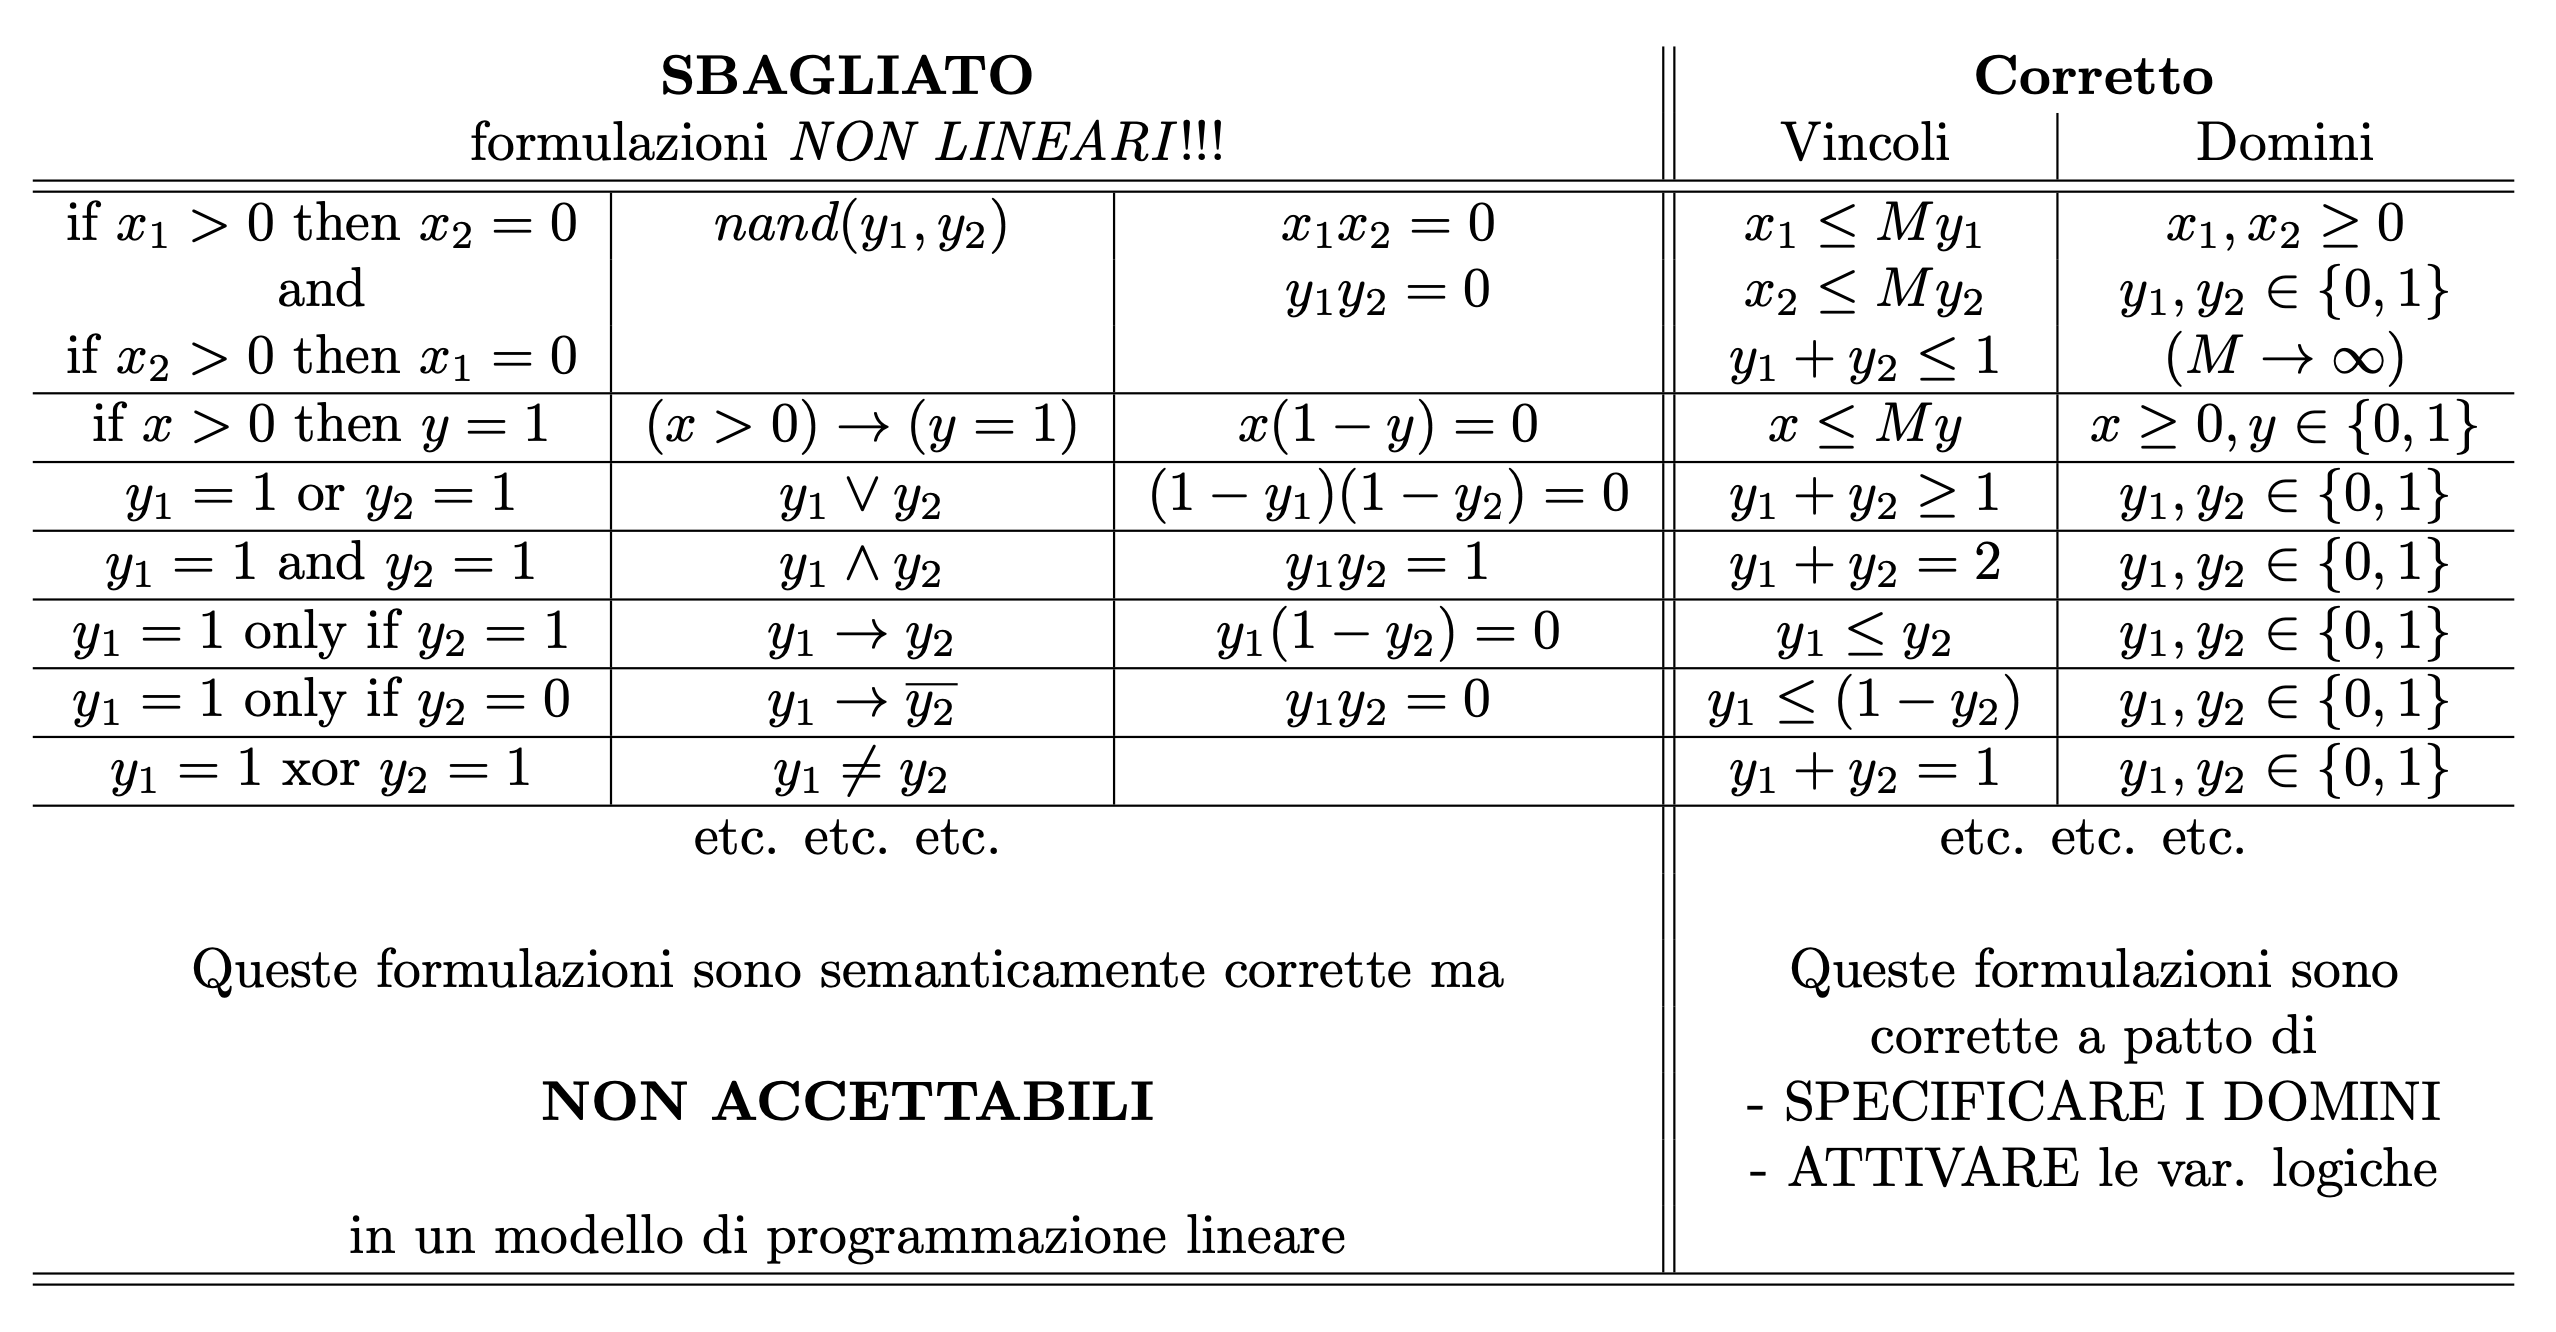
\includegraphics[width=0.5\textwidth]{log_var_table.png}
        \end{center}


